\documentclass[class=NCU_thesis_en, crop=false]{standalone}
\begin{document}

\chapter{Automatical write letters}
Here try to add some information to latters.(Now only support master Chinese letters)

\fontsize{10}{15}\selectfont % 影響字體位置,但只有行高有作用,字體大小照class設定,使用10pt對齊。

% \placetextbox{x(mm)}{y(mm)}  (0,0)at left bottom

\sffamily
% 碩博士論文電子檔授權書
\IfFileExists{letter_authorization.pdf}{
\cleardoublepage\thispagestyle{empty}
\includepdf[pagecommand={   \placetextbox{70}{95}{\LARGE\deptshort}%
                            \placetextbox{95}{105}{\LARGE\mprof}%
                            \placetextbox{100}{115.5}{\LARGE\title}}]%
{letter_authorization.pdf}}{}
% 碩博士紙本論文延後公開/下架申請書。(如需延後公開者,才需要裝訂於論文內頁)
\IfFileExists{letter_publication_request.pdf}{
\cleardoublepage\thispagestyle{empty}
\includepdf[pagecommand={   \placetextbox{70}{255}{\LARGE\deptshort}%
                            \placetextbox{123}{267}{\LARGE\author}%
                            \placetextbox{90}{216}{\LARGE\mprof}%
                            \placetextbox{100}{229}{\LARGE\title}}]%
{letter_publication_request.pdf}}{}
% 指導教授推薦書
\IfFileExists{letter_recommendation.pdf}{
\cleardoublepage\thispagestyle{empty}
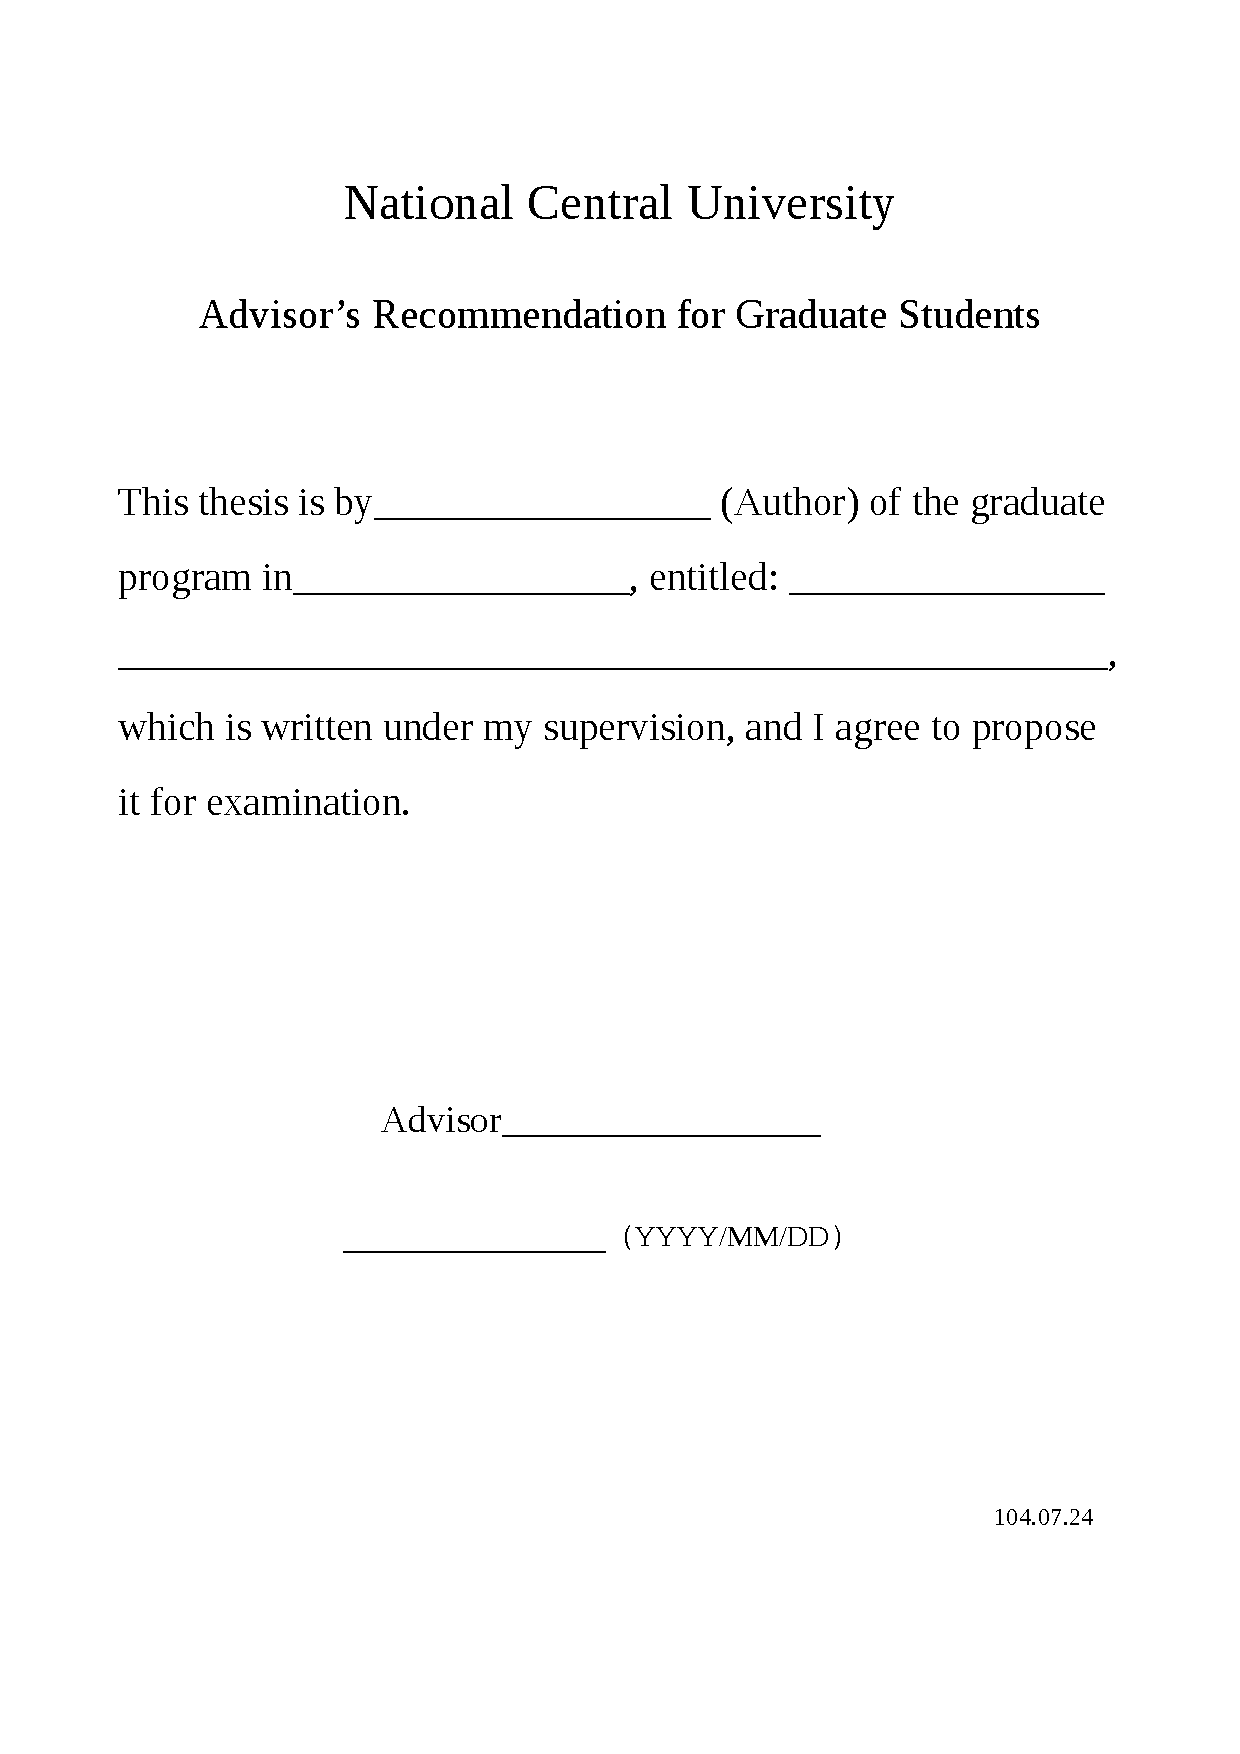
\includepdf[pagecommand={   \placetextbox{50}{157}{\huge\deptshort}%
                            \placetextbox{118}{157}{\huge\author}%
                            \placetextbox{105}{141}{\huge\title}}%
]{letter_recommendation.pdf}}{}
% 口試委員審定書
\IfFileExists{letter_verification.pdf}{
\cleardoublepage\thispagestyle{empty}
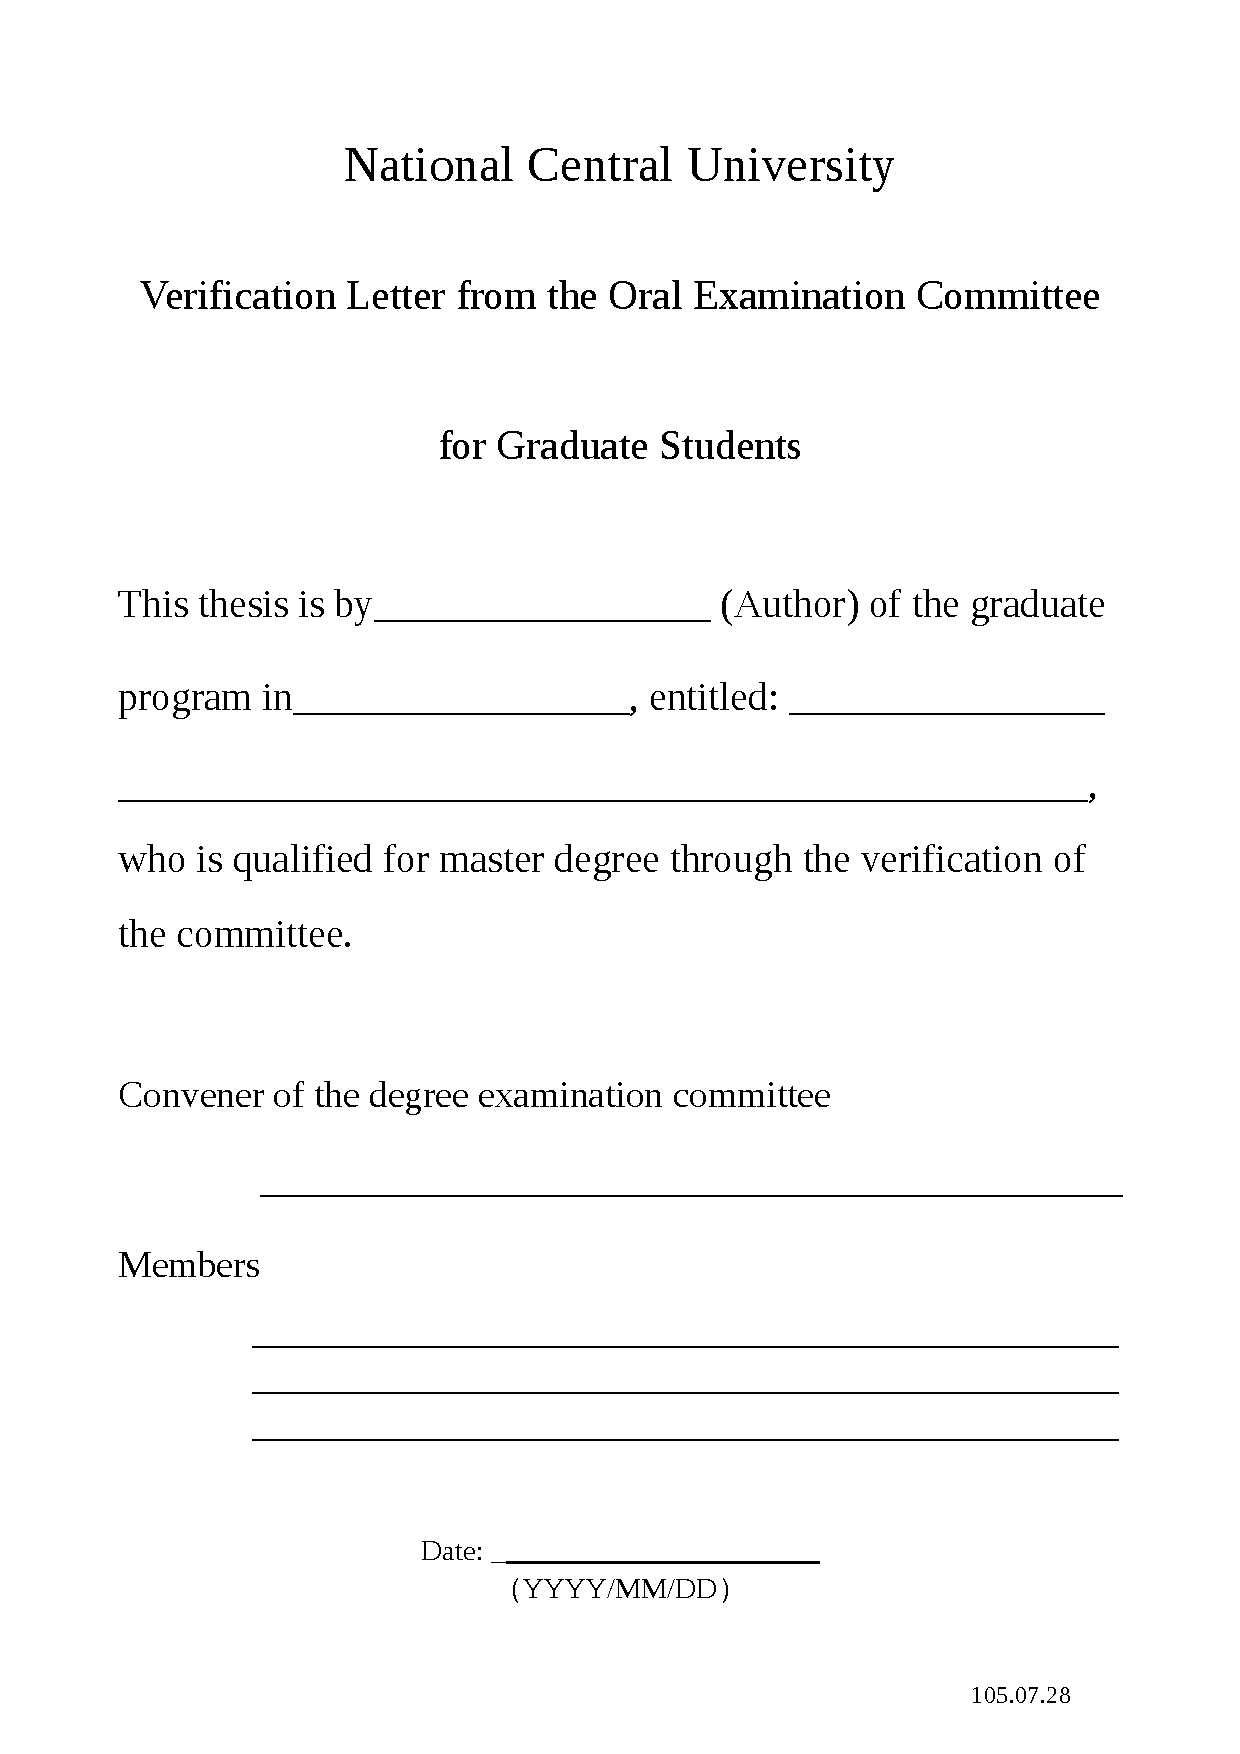
\includepdf[pagecommand={   \placetextbox{65}{198}{\huge\deptshort}%
                            \placetextbox{143}{198}{\huge\author}%
                            \placetextbox{100}{166}{\huge\title}}%
]{letter_verification.pdf}}{}
\end{document}